\thispagestyle{empty}
\vspace*{1.4cm}
\begin{center}
{\fontsize{32pt}{44pt}\selectfont\bfseries\textcolor{navy}{芯绘丹青}}\par
\vspace{.45cm}
{\fontsize{17pt}{26pt}\selectfont 端侧实时艺术渲染}\par
\vspace{.3cm}
{\large 基于Ti60 FPGA的十风格视频渲染系统}\par
\vspace{1.15cm}
{\Large\bfseries 技术报告}\par
\vspace{1cm}
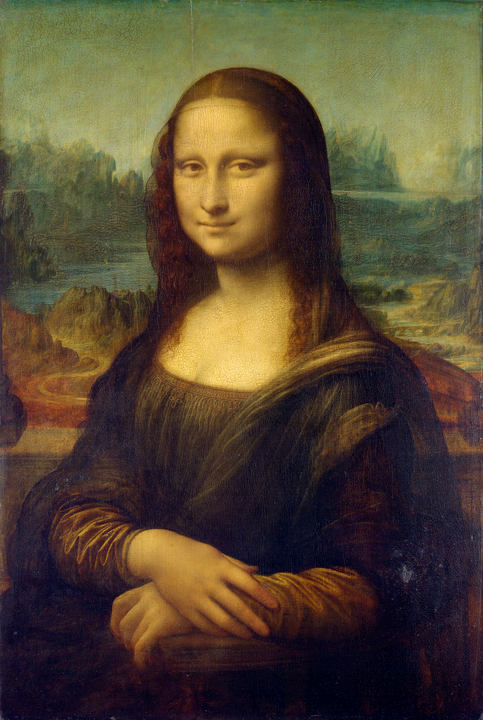
\includegraphics[height=4.2cm]{assets/comparisons/mona_lisa_original.png}\hspace{.25cm}
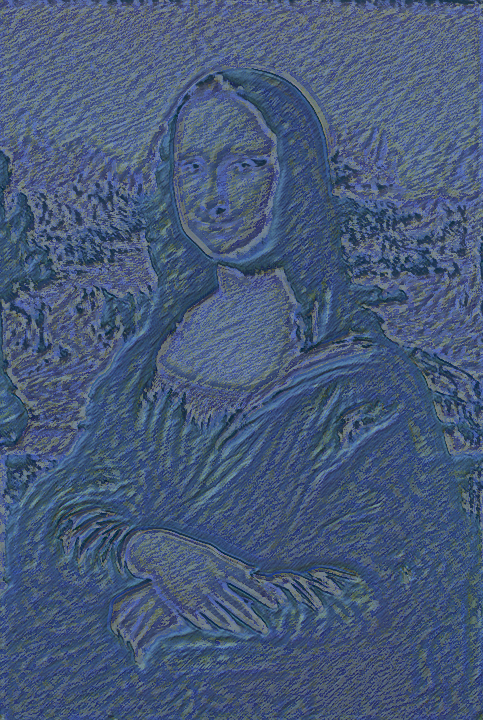
\includegraphics[height=4.2cm]{assets/comparisons/mona_lisa_00.png}\hspace{.25cm}
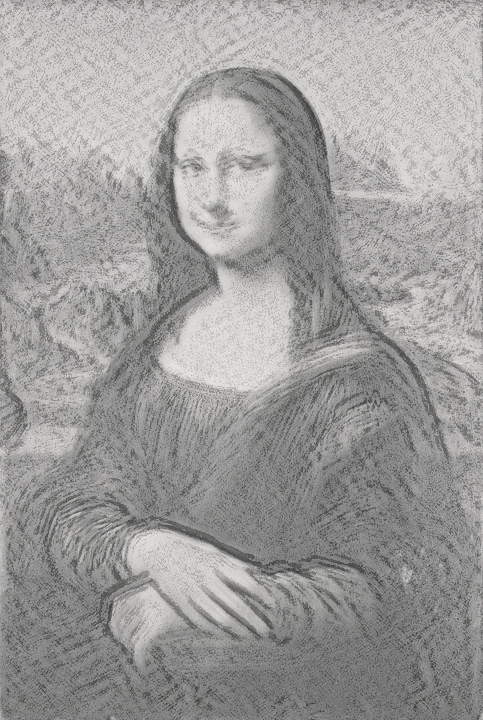
\includegraphics[height=4.2cm]{assets/comparisons/mona_lisa_04.png}\par
\vspace{.2cm}
{\small 原图\hspace{2cm}梵高厚涂\hspace{1.8cm}水墨}\par
\vspace{.25cm}
{\footnotesize 展示图来自当前学生模型的真实整数预测}\par
\vfill
\begin{tabular}{rl}
赛题方向 & AI赋能的“实时绘画”风格化视频渲染\\[5pt]
实现平台 & Ti60F225I3 DemoBoard V4 / SC431HAI\\[5pt]
工程版本 & \sig{camera_art_ten_paint}\\[5pt]
报告日期 & 2026年11月3日
\end{tabular}
\end{center}
\vspace*{.7cm}
\clearpage
\noindent{\fontsize{20pt}{28pt}\selectfont\bfseries\textcolor{navy}{项目速览}}\par
\noindent{\large 摄像头采集 → FPGA风格化 → HDMI呈现}\par
\smallskip

系统将SC431HAI的1080p RAW10视频转换为1280×720 RGB565，写入DDR3后由六通道卷积加速器处理。十组独立风格参数复用一套硬件，RISC-V负责传感器初始化、参数装载、作业与手势控制。网络各层保持720p，显示支持原图、风格图及同源左右对比。

\begin{figure}[H]\centering
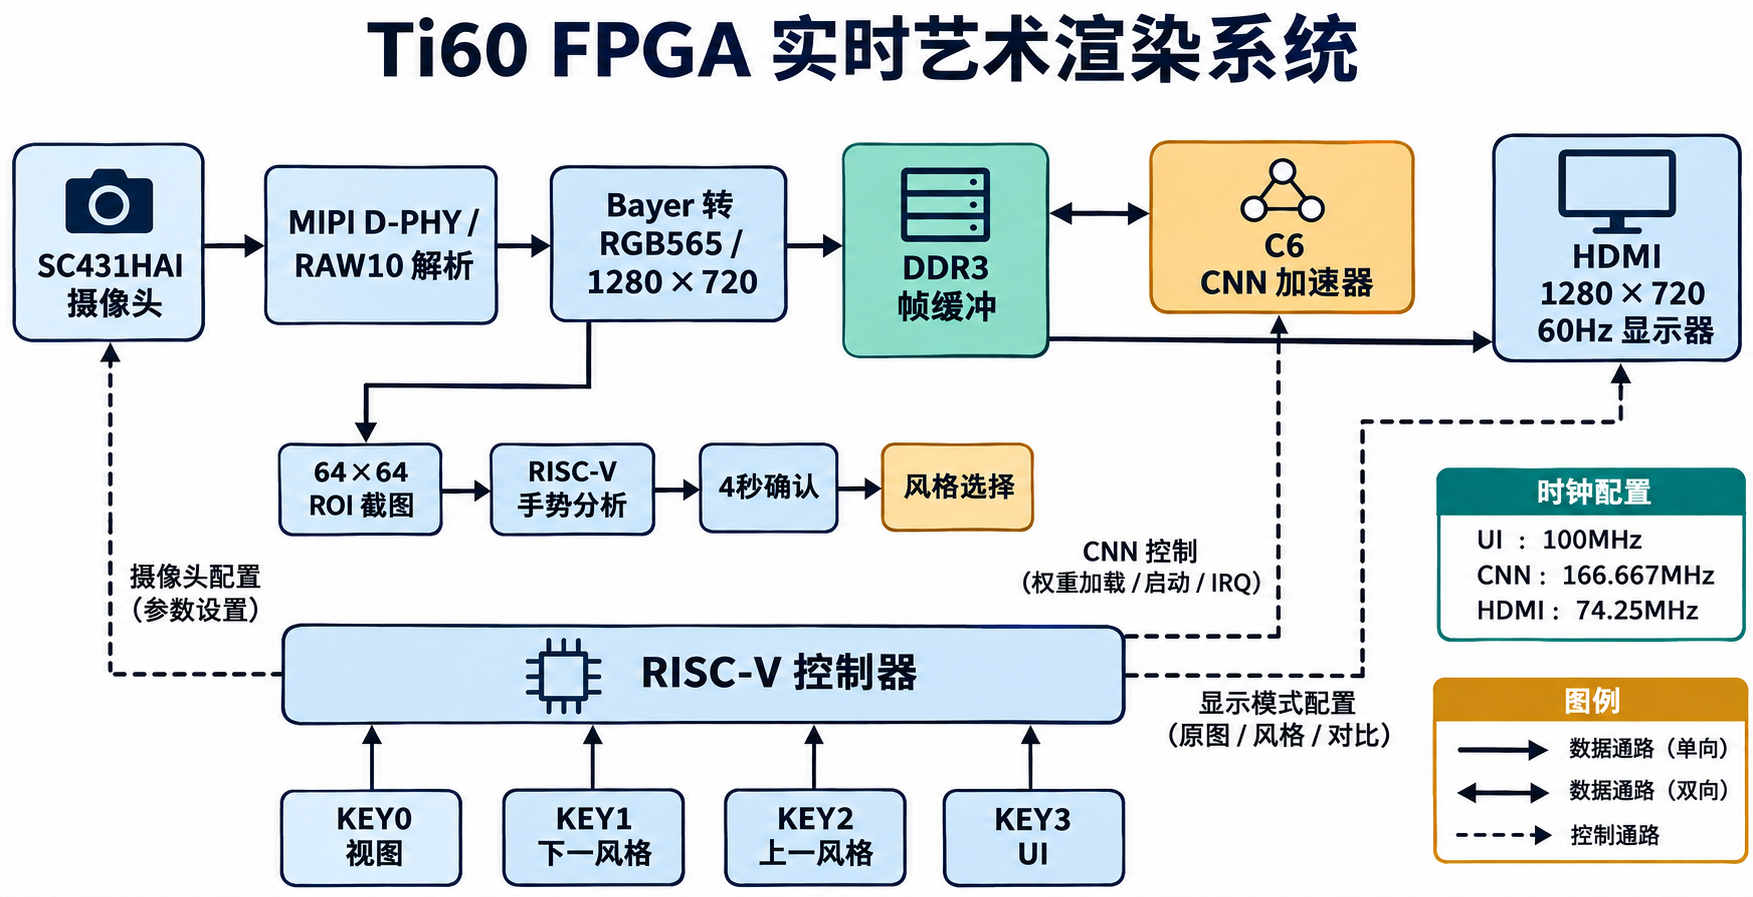
\includegraphics[width=.96\linewidth]{assets/generated/system.png}
\caption{系统总览：数据在DDR中交换，控制经APB传递；板载手势当前使用个人模板。}
\label{fig:system}
\end{figure}

\noindent\begin{tabularx}{\linewidth}{@{}p{.24\linewidth}X@{}}\toprule
核心指标 & 当前实现与证据\\\midrule
图像与显示 & 全1280×720处理；HDMI标准720p60刷新\\
轻量网络 & C6 / RF31；396个卷积权重/风格；十风格ROM 7360B\\
吞吐与资源 & CNN/DMA模型39.085fps；RAM230/256、DSP142/160\\
时序与边界 & setup/hold余量+0.108/+0.026ns；持续板上FPS待量化复测\\\bottomrule
\end{tabularx}
\medskip

\noindent\textbf{一帧流程：}好帧发布 → 锁住源bank → 加载216项参数（需要时）→ 四条带卷积 → 最后DDR写响应 → 安全消隐换帧。三源、三输出槽允许采集、计算和显示重叠。

\smallskip\noindent\textbf{交互方式：}KEY0切换视图，KEY1/KEY2切换风格，KEY3开关UI；在原图/对比界面识别手势0--9，持续四秒确认，原图确认后自动进入风格图。

\smallskip\noindent\textbf{成果范围：}当前bit完成CAD、定点与模块验证；20组名画输出为真实模型预测。免录入通用手势、外部在线权重下载以及持续整机30fps实测仍是后续工作。
